\documentclass{article}
\usepackage{booktabs}
\usepackage{amsmath}
\usepackage{amssymb}
\usepackage[noend]{algorithmic}
\usepackage[nothing]{algorithm}
\usepackage{tikz}
\usepackage{latexsym}
\usepackage{float}
\usetikzlibrary{arrows,automata}
\providecommand{\e}[1]{\ensuremath{\times 10^{#1}}}
\renewcommand{\thealgorithm}{}
\renewcommand*{\thefootnote}{[\arabic{footnote}]}
\title{CS 525: Theory of Computation\\ Final Exam}
\author{Dustin Ingram}
\begin{document}
\maketitle
\begin{enumerate}
    \item \textbf{Solution:}
        \begin{enumerate}
            \item The variables in $G$ are $\{R, S, T, X\}$. The terminals in $G$ are $\{a, b, \epsilon\}$. The start variable is $R$.
            \item Two strings in $G$ are `ab' and `ba'. A string not in $G$ is `a'.
            \item True.
            \item This language ensures that every string contains at least one `a' and one `b', and that for at least one character in the string $\{c_{1}, c_{2}, \dots, c_{n}\}$ there is a character at some $c_{i}$ such that the character at $c_{n-i}$ is the opposite.
        \end{enumerate}
    \item \textbf{Solution:}
        \begin{figure}[!h]
            \centering
            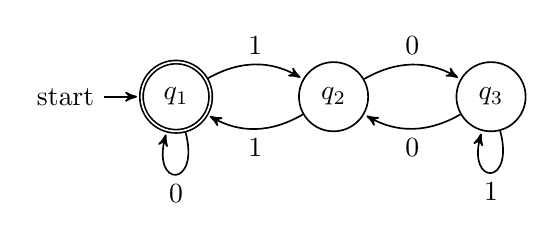
\begin{tikzpicture}[->,>=stealth',shorten >=1pt,auto,node distance=2.8cm,semithick]
              \node[state, initial, accepting]     (q1) at (0,0)  {$q_{1}$};
              \node[state]     (q2) at (2,0)  {$q_{2}$};
              \node[state]     (q3) at (4,0) {$q_{3}$};

              \path (q1) edge[bend left] node {$1$} (q2)
                    (q2) edge[bend left] node {$1$} (q1)
                    (q2) edge[bend left] node {$0$} (q3)
                    (q3) edge[bend left] node {$0$} (q2)
                    (q3) edge[loop below] node {$1$} (q3)
                    (q1) edge[loop below] node {$0$} (q1);
            \end{tikzpicture}
        \end{figure}

    \item \textbf{Solution:}
        \begin{enumerate}
            \item \textbf{intersection}: Let $M_{A}$ and $M_{B}$ be turing machines that accept languages $A$ and $B$, respectively. Construct a third machine, $M_{C}$, as follows: \\ \\
            $M_{C} = $ On input $\langle w \rangle$: 
            \begin{enumerate}
                \item Run $M_{A}$ on $w$. If $M_{A}$ halts and rejects, \emph{reject}, otherwise continue; 
                \item Run $M_{B}$ on $w$. If $M_{B}$ halts and rejects, \emph{reject}. If it accepts, \emph{accept}.
            \end{enumerate}

            \item \textbf{concatenation}: Let $M_{A}$ and $M_{B}$ be turing machines that accept languages $A$ and $B$, respectively. Construct a third machine, $M_{C}$, as follows: \\ \\
            $M_{C} = $ On input $\langle w \rangle$: 
            \begin{enumerate}
                \item Non-deterministically partition $w$ into every possible pair of substrings $\{w_{1}$, $w_{2}\}$;
                \item For every pair $\{w_{1}, w_{2}\}$, run $M_{A}$ on $w_{1}$ and $M_{B}$ on $w_{2}$;
                \item If, for any pair, $M_{A}$ accepts $w_{1}$ and $M_{B}$ accepts $w_{2}$, \emph{accept};
                \item Otherwise, \emph{reject}.
            \end{enumerate}

            \item \textbf{star}: Let $M_{A}$ be a turing machine that accepts $L(A)$. Construct a second machine, $M_{A^{*}}$ as follows:
            $M_{A^{*}} = $ On input $\langle w \rangle$: 
            \begin{enumerate}
                \item Non-deterministically partition $w$ into every possible set of non-empty substrings $\{w_{1}$, $w_{2}\, \dots, w_{n}\}$;
                \item Run $M_{A}$ on all $w_{i} \in$ all possible partitions;
                \item If, for any partition $M_{A}$ accepts all $w_{i}$ in the partition, \emph{accept}, otherwise \emph{reject}.
            \end{enumerate}
        \end{enumerate}
    \item \textbf{Solution:}
        To show $S_{DFA}$ is decidable, construct a new DFA $M^{\mathcal{R}}$ that accepts the reverse language $L^{\mathcal{R}}$ as follows:
        \begin{enumerate}
            \item Reverse the directions of all transitions in $M$;
            \item Create a new start state, with $\epsilon$-transitions from this state to all accepting states in $M$;
            \item Make the start state of $M$ the accepting state of $M^{\mathcal{R}}$
            \item Transform the resulting NFA into the DFA $S_{DFA}$.\footnote{Theorem 1.39, pg. 55}
        \end{enumerate}
    \item \textbf{Solution:}
        $L = \{\langle M, N\rangle|M, N$ are turing machines, $M$ uses an oracle to determine if $N$ is empty\} 

    \item \textbf{Solution:}
        \begin{enumerate}
            \item Construct a machine $M$ as follows: \\ \\
            $M = $ On input $\langle G, a, b, k \rangle$:
                \begin{enumerate}
                    \item If $k=0$, \emph{reject};
                    \item For each node $c$ adjacent to $a$ that has not already been considered:
                    \begin{enumerate}
                        \item If $b$ is $c$, \emph{accept};
                        \item Otherwise run M on $\langle G, c, b, k-1 \rangle$, if it accepts, \emph{accept}.
                    \end{enumerate}
                    \item Otherwise, \emph{reject}.
                \end{enumerate}
            \item Assume $M$ decides LPATH in polynomial time. Then we can construct a DFA $M^{\prime}$ which can decide HAMPATH in polynomial time as follows: \\ \\
            $M^{\prime} = \langle G, a, b \rangle$:
            \begin{enumerate}
                \item Run $M\langle G, a, b, n \rangle$, where $n$ is the number of nodes in $G$;
                \item If $M$ accepts, \emph{accept}, otherwise \emph{reject}.
            \end{enumerate}
            This is contradictory, as we know HAMPATH is NP-complete.\footnote{Theorem 7.46, pg. 286}
        \end{enumerate}
\end{enumerate}
\end{document}
